%\documentclass[final,hyperref={pdfpagelabels=false}]{beamer}
\pdfminorversion=4
\documentclass[xcolor=dvipsnames]{beamer}



%Load the myriad packages
\usepackage{xcolor}
\usepackage{subcaption}
\usepackage{tikz}
\usetikzlibrary{shapes.geometric, arrows}
\tikzstyle{startstop} = [rectangle, rounded corners, minimum width=2cm, text
    width=1.8cm, minimum height=1cm,text centered, text=white,draw=black, fill=Gray!140]
\tikzstyle{io} = [trapezium, trapezium left angle=70, trapezium right angle=110,
minimum width=0.5cm, minimum height=1cm, text centered, draw=black,
fill=blue!20!Gray!90!,text=white]
\tikzstyle{process} = [rectangle, minimum width=2cm, minimum height=1cm, text
centered, text width=2cm, draw=black, text=white,fill=Gray!140!blue!70!white]
\tikzstyle{decision} = [diamond, minimum width=2.0cm, minimum
    height=0.81cm,aspect=1.40, text centered, draw=black, fill=Gray!,text=white]
\tikzstyle{arrow} = [thick,line width=0.5mm,->,>=stealth]
\tikzstyle{arrow1} = [dashed,->,>=stealth]

%Math commands
\newcommand{\deriv}[2]{\frac{\mathrm{d} #1}{\mathrm{d} #2}}
\newcommand{\pderiv}[2]{\frac{\partial #1}{\partial #2}}
\newcommand{\bx}{\mathbf{X}}
\newcommand{\ba}{\mathbf{A}}
\newcommand{\by}{\mathbf{Y}}
\newcommand{\bj}{\mathbf{J}}
\newcommand{\bs}{\mathbf{s}}
\newcommand{\B}[1]{\ensuremath{\mathbf{#1}}}
\newcommand{\Dt}{\Delta t}
\renewcommand{\d}{\mathsf{d}}
\newcommand{\mom}[1]{\langle #1 \rangle}
\newcommand{\xl}{{x_{i-1/2}}}
\newcommand{\xr}{{x_{i+1/2}}}
\newcommand{\il}{{i-1/2}}
\newcommand{\ir}{{i+1/2}}

%other commands
\renewcommand{\u}[1]{\underline{#1}}
\newcommand{\iso}[2]{${}^{{#2}}${#1} }
\newcommand{\expect}[1]{E[#1] }
\newcommand{\colg}[1]{{\color{ForestGreen} #1}}
\newcommand{\coly}[1]{{\color{yellow} #1}}
\newcommand{\colw}[1]{{\color{white} #1}}
\newcommand{\colb}[1]{{\color{blue} #1}}
\newcommand{\colr}[1]{{\color{red} #1}}

\usepackage{amssymb,amsmath}
\usepackage[english]{babel}
\usepackage[latin1]{inputenc}
\usepackage[orientation=portrait,size=a0,scale=1.4]{beamerposter}
\usepackage{textcomp}
\usepackage{varwidth}
\usepackage{graphicx}
%\usepackage{tikz}
%\usepackage[numbers, super]{natbib}
\usepackage{grffile} %spaces in file names
\usepackage{parskip}
%\usepackage[T1]{fontenc} %for sc and bf
%\usepackage{times}
\usepackage{wasysym}
\usepackage{bigstrut}
\usepackage{float}
\usepackage{setspace}
%\usepackage{enumitem}
%\setlist{nolistsep} % or \setlist{noitemsep} to leave space around whole list
% Load some optional sub-parts of PGF
%\usetikzlibrary{decorations.pathmorphing}
%\usetikzlibrary{positioning}
%\usetikzlibrary{calc}
%\usetikzlibrary{shapes.geometric}
%\usepackage{pgfplots}

%misc.
\newcommand{\nn}[1]{\ensuremath{^{#1}}} %[1] is # of commands
\newcommand{\keff}{\ensuremath{{k_\mathrm{eff}}}}
\newcommand{\kinf}{\ensuremath{{k_\infty}}}
\newcommand{\alphaT}{\ensuremath{{\alpha_{_T}}}}
\newcommand{\SN}{\ensuremath{{\text{S}_\text{N}}}}
%Note: tarticle has ``several'' changes from article
%in this vein.
% some simplifying commands

\newcommand{\eg}{{\it e.g.}}
\newcommand{\ie}{{\it i.e.}}
\newcommand{\etal}{{\it et al.\,}}
\newcommand{\acite}[1]{{\bf(Add Citation: #1)}}
\newcommand{\E}{\mathcal{E}}
% derivative - d
\newcommand{\ud}{\,\mathrm{d}}
% bold unit vector n-hat
\newcommand{\nhat}{\hat{\bf n}}
\newcommand{\tensor}[1]{\mathcal{#1}}
\renewcommand{\vec}[1]{\mathbf{#1}}
\newcommand{\om}{\boldsymbol{\Omega}}
%


\definecolor{myblue}{rgb}{0.7, 0.7, 60.0}


\newcommand\highlight[1]{%
          \colorbox{myblue!32}{\begin{varwidth}{\dimexpr\linewidth-2\fboxsep}#1\end{varwidth}}}




\graphicspath{{../images/}}
%\listfiles
%\boldmath

%%%%%%%%%%%%%%%%%%%%%%%%%%%%%%%%%%%%%%%%%%%%%%%%%%%%%%%%%%%%%%%
% Optional packages, used to show off certain tricks

\newlength \figwidth
\setlength \figwidth {0.5\textwidth}

%%%%%%%%%%%%%%%%%%%%%%%%%%%%%%%%%%%%%%%%%%%%%%%%%%%%%%%%%%%%%%%

\mode<presentation>
{
   \usetheme{TAMU}
}

\title{\color{black}A High-Order Low-Order Algorithm with Residual \\ Monte Carlo Time
Integration for Radiative Transfer}

\author{\large Simon~R.~Bolding \& Jim~E.~Morel}

%TAMU
\institute{Department of Nuclear Engineering,
Texas A\&M University -- CERT Project}

% You can override the default acknowledgment, and address if you want
%\acknowledgement{*Submitted in partial fulfillment of the requirements of NUEN 610 \\
%(Nuclear Reactor Design)}
%\address{Nuclear Engineering Department \\
%            Texas A\&M University \\
%            College Station, TX 77843-3133}}

% If you don't want the menu section outline above the title, do this:
%\setbeamertemplate{headline}{}

\newlength{\columnheight}
\setlength{\columnheight}{105cm}

%%%%%%%%%%%%%%%%%%%%%%%%%%%%%%%%%%%%%%%%%%%%%%%%%%%%%%%%%%%%%%%%%%%%%%%%%%%%%%%%%%%%%%%%%%%%%
\begin{document}
\begin{frame}
\begin{columns}

    % ---------------------------------------------------------%
    % Set up a column
\begin{column}{.49\textwidth}
\begin{beamercolorbox}[center,wd=\textwidth]{postercolumn}
\begin{minipage}[T]{0.95\textwidth} % tweaks the width, makes a new \textwidth
\parbox[t][\columnheight]{\textwidth}{ % must be some better way to set the the height, width and textwidth simultaneously
         % Since all columns are the same length, it is all nice and tidy.  You have to get the height empirically
         %%%%%%%%%%%%%%%%%%%%%%%%%%%%%%%%%%%%%%%%%%%%%%%%%
       \begin{block}{Overview and background on thermal radiative transfer}
         \begin{itemize}
             \setlength{\itemsep}{0.6em}
             \item The continuous radiation and material energy
                 equations are
\begin{align}
    \frac{1}{c}\pderiv{I}{t} + \mu \pderiv{I}{x} + \sigma_t I(x,\mu,t)
    &= \frac{\sigma_s \phi(x)}{4\pi} +  \frac{1}{4\pi} \sigma_a a c T^4,\label{ho_trans}
  \\
  C_v \pderiv{T(x,t)}{t} &=  {\sigma_a \phi(x,t)} - {\sigma_a a c T^4} \label{lo_mat}
\end{align}
     \item The radiation intensity $I(x,\mu,t)$ and material temperature
         $T(x,t)$ are
         \textbf{coupled}
         through photon \textbf{emission} $\sigma_a a c T^4$ and
         \textbf{absorption} $\sigma_a \phi$.
      \item We form a \textbf{lower-dimensional} system which can
          efficiently \textbf{resolve non-linearities} in the problem.  The low-order
          (LO) equations contain consistency terms that preserve accuracy
          of \textbf{efficient}, high-order (HO) exponentially-convergent Monte Carlo (ECMC) simulations.
      \item[] \highlight{We now include the time variable $t$ in the MC transport
              algorithm with a \textbf{consistent} LO temporal closure.  \colb{This improves
              the accuracy of radiation wavefronts in optically thin problems.}}
      \end{itemize}
         \end{block}
         \vfill

         %%%%%%%%%%%%%%%%%%%%%%%%%%%%%%%%%%%%%%%%%%%%%%%%%
	\begin{block}{The HOLO algorithm is applied for each time step}
        \resizebox{0.9618\linewidth}{!}{
    \fontsize{10}{11.0}\selectfont
    \begin{tikzpicture}[node distance=2cm]
        \node (start) [startstop] {Initialize LO system with $I^n$};
        \node (in1) [process, right of=start, xshift=2cm, text width=3.3cm]  {{}
        \colw{LO Newton solve, fully converged}};%{LO solve:\vspace{0.041in}        $\B D(\mu^{HO})\Phi = \frac{1}{\keff}\B F\Phi$};
        \node (pro1) [io, below of=in1] {$T_{LD}^{n+1}(x)$, $\phi_{LD}^{n+1}(x)$};
        \node (dec1) [decision, below of=pro1, yshift=-0.5cm, text width=1.74cm] {Outer Converged?};
        \node (pro2a) [process, left of=dec1, xshift=-2.0cm] {Move to the next time step};
        \node (srcs) [process, right of=dec1, xshift=3.0cm, text width=2.8cm] {{{}}
        \colw{Construct LD emission source}};
        \node (pro2b) [process, above of=srcs, yshift=0.5cm] { \colw{HO solve
        for $\tilde I(x,\mu,t)$}};
        \node (cons) [process, above of=pro2b, text width=3.0cm] {\colw{Consistency
        terms}};
        \draw [arrow1] (start) -- (in1);
        \draw [arrow] (in1) -- (pro1);
        \draw [arrow] (pro1) -- (dec1);
        \draw [arrow] (srcs) -- (pro2b);
        \draw [arrow] (dec1.east) -- node[anchor=south] {no} (srcs);
        \draw [arrow1] (dec1.west) -- node[anchor=south] {yes} (pro2a);
        \draw [arrow1] (pro2a) -- (start);
        \draw [arrow] (pro2b) -- (cons);
        \draw [arrow] (cons) -- (in1);
    \end{tikzpicture}
}
	\end{block}
	\vfill
         \vfill
         %%%%%%%%%%%%%%%%%%%%%%%%%%%%%%%%%%%%%%%%%%%%%%%%%%%%%%%%%
         \begin{block}{Details of the LO equations} 
         \setlength\itemsep{0.2em}
            \begin{itemize}
                \item The LO equations are formed with spatial, angular, and temporal
                    moments of Eq.~\eqref{ho_trans} \& ~\eqref{lo_mat} and algebraic
                    manipulation. Moments are defined locally over the $i$-th spatial finite element (FE) and 
                    $n$-th time step. \vspace{0.2em}
        \end{itemize}
       \begin{minipage}{0.45\textwidth}
        \centering
        \resizebox{0.99\linewidth}{!}{
            {\tiny
                \begin{tikzpicture}[scale=1.3]
 %                   \node at (3.2105,6.00) {\tiny \colb{Spatial Element $i$}};
                    \draw (0.8,5.0) -- (1.2,5.0) node[anchor=east]{$1$ \hspace{0.4em} };
            \draw (1.0,0.4) -- (1.0,0.6) node[below, pos=0.4] {$x_{i-1/2}$};
            \draw (5.90,0.4) -- (5.90,0.6) node[below, pos=0.4] {$x_{i+1/2}$};
            \node at (4.8,5.0) {$b_{R,i}(x)$};
            \node at (2.0,5.0) {$b_{L,i}(x)$};
            \draw [thick,->] (-0.5,0.5) -- (7.0,0.5) node[anchor=north west] {$x$};
            \draw [dashed,->] (5.90,0.5) -- (5.90,5);
            \draw [dashed,->] (1.0,0.5) -- (1.0,5.5);
            \draw (1.0,0.5) -- (5.90,5.0);
            \draw (5.90,0.5) -- (1.0,5.0);
        \end{tikzpicture}
    }
}
%       \begin{figure}
%    \begin{centering}
%        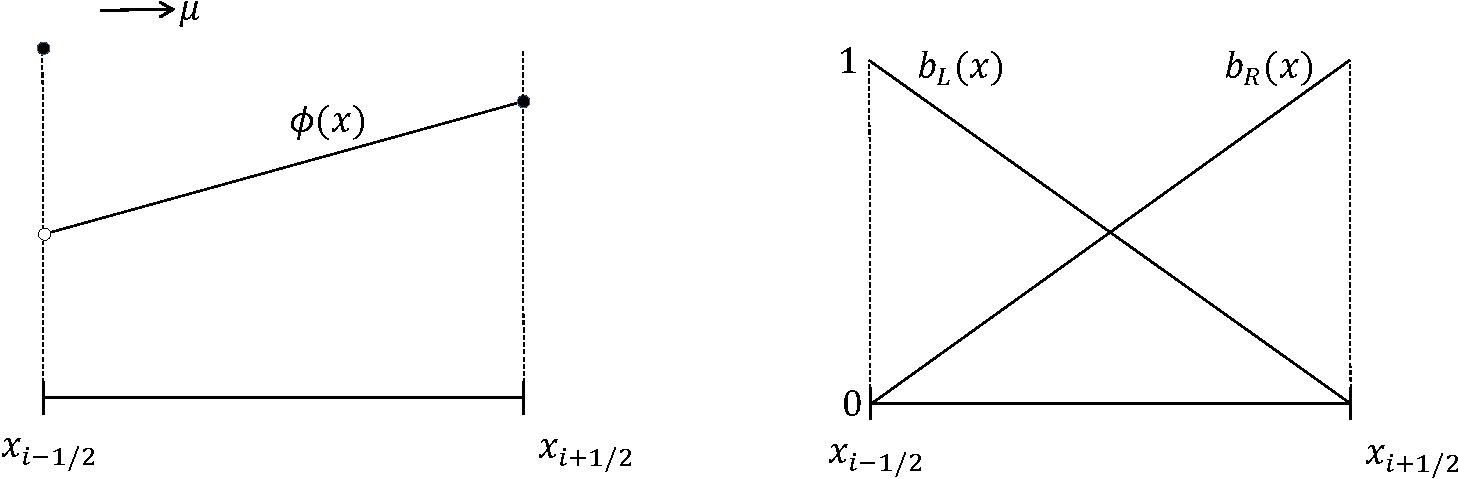
\includegraphics[trim=5.0in 0.0in 0.0in 0.0in,clip,width=0.9\textwidth]{LD.pdf}
%    \end{centering}
%    \end{figure}
    \end{minipage}
    \begin{minipage}{0.45\textwidth}
    \begin{center}
        {\small
    \begin{tabular}{c}
        \underline{Spatial moments} \\[1em]
        $ {\displaystyle \mom{\cdot}_{L/R,i} = \frac{2}{h_i} \int_{x_\il}^{x_\ir}
        b_{L/R,i}(x)(\cdot) \d x \quad }$ \vspace{0.4in} \\[1em]  \underline{Angular half-ranges}
        \\[1em] ${ \quad \displaystyle \phi^\pm(x) =
            \pm\int_0^{\pm 1} I(x,\mu) \d \mu}$ \vspace{0.3in}
\end{tabular}}
    \end{center}
\end{minipage}
    \begin{itemize} 
        \item The space-angle moment equations are exactly integrated over the $n$-th time
            step.  Temperature unknowns must be discretized with linear-discontinuous
            finite elements (LDFE) in space and backward
            Euler in time.
        \setlength\itemsep{0.5em}
\item We use the latest ECMC solution for the \textbf{time-averaged projection} of
    $I(x,\mu,t)$ to evaluate \colb{angular consistency terms} in the LO equations, e.g.,
        \begin{equation*}
            \{\overline \mu\}^{+}_{L,i} = \frac{\mom{\mu\, \overline I_{HO}\left( x,\mu \right)}_{L,i}^+}{\mom{\overline
                I_{HO}\left(x,\mu\right)}_{L,i}^+}
        \end{equation*}
        \item The extra end-of-time-step radiation moments, i.e., $\phi^{n+1}$, are
            eliminated in terms of time-averaged moments, i.e., $\overline \phi$, with
            \textbf{parametric time closures}.  The ECMC solution is used to estimate the
            \colb{local     closures}, e.g.,
            \begin{equation*}
                \mom{\phi}_{L,i}^{n+1,+} = {\gamma^{HO,+}_{L,i}} {\mom{\overline{\phi}}}^+_{L,i} 
            \end{equation*}
            where $\gamma^{HO,+}_{L,i}$ is a constant that is estimated with the above relation and the
            HO solution.  There is a time closure for each radiation moment equation.
        \item  The nonlinearities are fully resolved \emph{for each LO solve} using \colb{Newton's
method,} based on the current HO consistency terms and time closure.

        \item The equations are solved in terms of time-averaged unknowns, then the
            solution is advanced to $t^{n+1}$ for the next time step
            using the time closure.
    \end{itemize}
\end{block}

%%%%%%%%%%%%%%%%%%%%%%%%%%%%%%%%%%%%%%%%%%%%%%%%%%%%%%%%%
\vfill
%%%%%%%%%%%%%%%%%%%%%%%%%%%%%%%%%%%%%%%%%%%%%%%%%%%%%%%%%%%%%
    \begin{block}{Acknowledgements}
        \begin{figure}
            \centering
            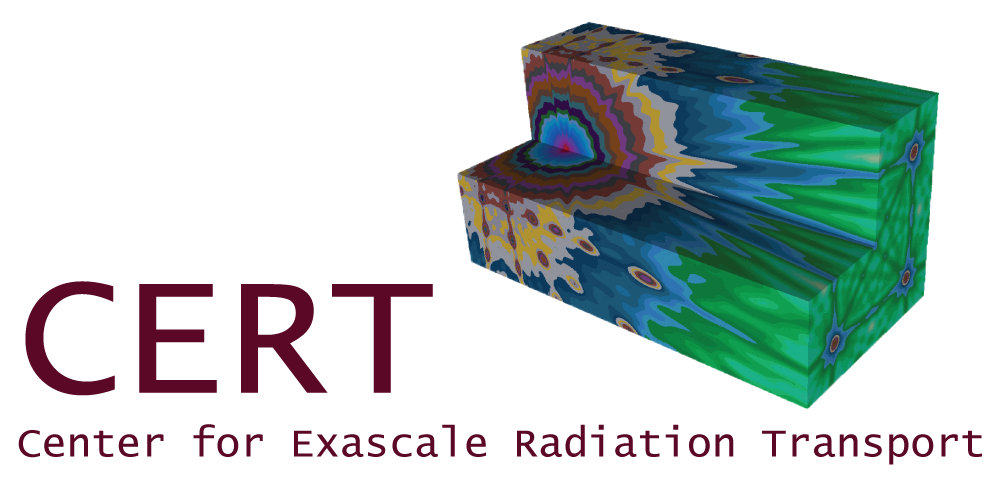
\includegraphics[width=0.25\textwidth]{cert_logo_maroon.png}
     \end{figure}
    \end{block}
    %%%%%%%%%%%%%%%%%%%%%%%%%%%%%%%%%%%%%%%%%%%%%%%%%
}
\end{minipage}
\end{beamercolorbox}
\end{column}
\begin{column}{.49\textwidth}
\begin{beamercolorbox}[center,wd=\textwidth]{postercolumn}
\begin{minipage}[T]{0.95\textwidth} % tweaks the width, makes a new \textwidth
\parbox[t][\columnheight]{\textwidth}{ % must be some better way to set the the height, width and textwidth simultaneously
         % Since all columns are the same length, it is all nice and tidy.  You have to get the height empirically
    %%%%%%%%%%%%%%%%%%%%%%%%%%%%%%%%%%%%%%%%%%%%%%%%%
    %%%%%%%%%%%%%%%%%%%%%%%%%%%%%%%%%%%%%%%%%%%%%%%%%
 %   \begin{columns}
 %       \column{0.015\textwidth}
 %       \column{0.47\textwidth}
        %
 %       \begin{block}{High-fidelity weighting function}
 %       \centering
 %       %\includegraphics[width=\figwidth]{../results/images/p1/e1/refWgt/base/p_effsigt.pdf} \\
 %       {\small Region-averaged reference solution} \\
 %       \end{block}
 %       %
 %       \column{0.025\textwidth}
 %       \column{0.47\textwidth}
 %       \begin{block}{Low-fidelity weighting function}
 %       \centering
 %       %\includegraphics[width=\figwidth]{../results/images/p1/e1/NJOYwgt/base/p_effsigt.pdf} \\
 %       {\small Essentially $1/E$} \\
 %       \end{block}
 %   \end{columns}
 %   \vfill
 %   %%%%%%%%%%%%%%%%%%%%%%%%%%%%%%%%%%%%%%%%%%%%%%%%%
 %  \begin{block}{ Better accuracy per DOF than standard MG}
 %     \centering
 %  \vspace{-3mm}
 %   Problem 4, Base problem, Errors in QOI
 %   \vspace{3mm}
 %   \begin{columns}[b]
 %   %
 %   \column{0.5\textwidth}
 %   \centering
 %   {\small Reference weighting }
 %   %\includegraphics[width=\figwidth]{../results/images/p4/e4/refWgt/base/p_common_err.pdf} \\
 %   %\includegraphics[width=\figwidth]{../results/images/p4/e4/refWgt/resonanceRes/p_common_res_k-eig.pdf} \\
 %   %
 %   \column{0.5\textwidth}
 %   \centering
 %   {\small Generic weighting }
 %   %\includegraphics[width=\figwidth]{../results/images/p4/e4/NJOYwgt/base/p_common_err.pdf} \\
 %   %\includegraphics[width=\figwidth]{../results/images/p4/e4/NJOYwgt/resonanceRes/p_common_res_k-eig.pdf} \\
 %   \end{columns}
 %   \end{block}

%%%%%%%%%%%%%%%%%%%%%%%%%%
\begin{block}{Details of ECMC Algorithm with MC time integration}
    \begin{itemize}
        \setlength\itemsep{0.5em}
        \item The HO emission source is constructed from the previous LO
            solution, producing a \textbf{fixed source,
            pure absorber} HO problem. 
        \item ECMC requires a trial space representation $\tilde I(x,\mu,t)$ for the
            intensity. \\  We use a
            \colb{step doubly discontinuous} space in $t$, with an LDFE projection
            in $x$ and $\mu$:
            \vspace{0.1in}
    \begin{center}
        \resizebox{0.48518\linewidth}{!}{
    \fontsize{12}{11.0}\selectfont
        \begin{tikzpicture}[scale=1.4, every node/.style={transform shape}]
            \node[anchor=south] at (1,4.0) {$\tilde{I}_{HO}^{n}(x,\mu)$};
            \draw (1.0,4.0) node[fill,circle,inner sep=0pt,minimum
            size=4.2pt] {};
            \draw [->] (4.3,4.25) -- (5.3,4.25) node[anchor=west] {$t$};
            \draw (1.0,0.4) -- (1.0,0.6) node[below, pos=0.4] {$t^{n}$};
            \draw (5.90,0.4) -- (5.90,0.6) node[below, pos=0.4] {$t^{n+1}$};
            \node at (3.6,3.06) {$\overline{I}_{HO}(x,\mu)$};
            \draw [thick] (1.0,0.5) -- (5.9,0.5) node[anchor=north west] {};
            \filldraw[color=black, fill=white] (1,2.450) circle (2.1pt);
            \draw (1.0,2.45) -- (5.90,2.45);
            \filldraw[color=blue, fill=white] (5.9,2.450) circle (2.1pt);
            \draw (5.9,1.6) node[blue,fill,circle,inner sep=0pt,minimum size=4.2pt] {};
            \node[anchor=west] at (5.9,1.6) {${\color{blue}\tilde{I}_{HO}^{n+1}(x,\mu)}$};
        \end{tikzpicture}
    }
    \end{center}
        \item The continuous time derivative $\frac{1}{c}\pderiv{}{t}\left(\cdot\right)$
            is included in the transport operator. With $T^4(x)$ implicit in time, the
            residual for $\tilde I(x,\mu,t)$ is
            \vspace{0.20in}
            \begin{equation*}
                r(x,\mu,t) = \frac{1}{2}\sigma_a^{n+1} a c \left(T^{n+1}\right)^4 -
                \frac{1}{c}\pderiv{\tilde I}{t} - \mu \pderiv{\tilde I}{x} - \sigma_a
                {\tilde I}
            \end{equation*}\vspace{-0.10in}
        \item Particle histories are sampled and tracked in time to get a MC solution to
            the transport
            equation for the error in $\tilde I(x,\mu,t)$.  The error is projected onto
            the trial space to accurately estimate the time-averaged and $t^{n+1}$
            intensities.
    \end{itemize}
\end{block}
    \vfill
    %%%%%%%%%%%%%%%%%%%%%%%%%%%%%%%%%%%%%%%%%%%%%%%%%
     %%%%%%%%%%%%%%%%%%%%%%%%%%%%%%%%%%%%%%%%%%%%%%%%%%%%%%%%%%%%%%%%%%%%%%%%%%%%%%%%
    \vfill
    \vfill
    \begin{block}{Computational Results}
    \begin{itemize}
        \setlength\itemsep{0.2em}
        \item The MC time integration with time closure (HOLO-TC) improves accuracy in optically thin problems compared
            to backward Euler time discretization (HOLO-BE). Figure depicts radiation temperature $T_R = \sqrt[4]{\phi/(ac)}$.
    \end{itemize}
    \vspace{0.7em}
    \centering \textbf{Optically thin problem:} $\sigma_a=0.2$ cm$^{-1}$
\begin{figure}
    \begin{subfigure}{\textwidth}
    \centering
    \includegraphics[width=0.65\textwidth]{thin_temp_compare.pdf}
    \caption{Radiation temperatures $T_R = \sqrt[4]{\phi/(ac)}$}
\end{subfigure}
\vspace{0.2in}
\end{figure}
    \begin{itemize}
        \item The HOLO method converges nonlinearites with damped Newton iterations to
            prevent artificial ``temperature spikes'' that IMC demonstrates.  Results below
            are the same problem but with different axis scales.
    \end{itemize}
    \vspace{0.3in}
\begin{figure}
\begin{subfigure}{0.49\textwidth}
    \centering
    \includegraphics[width=0.99\textwidth]{mpv_mats_imc.pdf}
    \caption{IMC temperatures for different $\Delta t$.\label{twomat_full}}
\end{subfigure} 
\begin{subfigure}{0.49\textwidth}
\centering
    \includegraphics[width=0.99\textwidth]{mpv_mats_holo.pdf}
    \caption{HOLO temperatures for different $\Delta t$.\label{twomat_quick}}
\end{subfigure}
\end{figure}
    \vspace{1.5em}
\centering 
    \end{block}

    %%%%%%%%%%%%%%%%%%%%%%%%%%%%%%%%%%%%%%%%%%%%%%%%%
     \vfill
    %%%%%%%%%%%%%%%%%%%%%%%%%%%%%%%%%%%%%%%%%%%%%%%%%
    \begin{block}{Ongoing work}
    \begin{itemize}
        \setlength\itemsep{0.25em}
        \item We are working towards a \colb{linear-discontinuous} trial space in time.  ECMC will be used to estimate
              the slope of the intensity in time, which can be used to extrapolate the
              solution to $t^{n+1}$. This  
              representation will improve the statistical efficiency over current tallies
              for $\tilde I^{n+1}(x,\mu)$ because all particles will contribute to the
              local slope.
        \item The LDFE $x$-$\mu$-$t$ space will require a more sophisticated sampling
            approach, which will be useful to investigate for extending
              ECMC to higher dimensions.
        \end{itemize}
    \end{block}
     \vfill
}
\end{minipage}
\end{beamercolorbox}
\end{column}

\end{columns}
\end{frame}
\end{document}

    %%%%%%%%%%%%%%%%%%%%%%%%%%%%%%%%%%%%%%%%%%%%%%%%%
    %\begin{block}{The transport equation}
    %\vspace{-16mm}
    %    \begin{align*}
    %    \small
    %    \om \cdot \nabla \psi(\vec{r}, E, \om) + \Sigma_t(\vec{r}, E) \psi(\vec{r}, E, \om) &= \frac{1}{4 \pi} \int_0^\infty \ud{E'} \Sigma_{s}(\vec{r}, E' \rightarrow E) \phi (\vec{r}, E') \;+ \nonumber \\
    %     &\qquad \frac{\chi(\vec{r}, E) }{4 \pi \, \keff} \int_0^\infty \ud{E'} \nu \Sigma_{f}(\vec{r}, E') \phi (\vec{r}, E')
    %    \end{align*}
    %    {
    %\footnotesize
    %With $\vec{r}$ the spatial coordinate, $E$ the energy, $\om$ the direction of travel, $\psi$ the radiation angular intensity, $\Sigma_t$ the total cross section, $\Sigma_s$ the scattering cross section, $\nu\Sigma_f$ the neutron production by fission cross section, $\keff$ the criticality eigenvalue, $\chi$ the fission distribution, and $\phi$ the scalar (angle-integrated) flux.
    %}
    %\end{block}
    %\vfill
